\begin{frame}
  \frametitle{\textbf{Charged Particle Suppression}}
  \begin{columns}
    \column{0.5\textwidth}
    \begin{itemize}
    \item Charged partons lose energy as they traverse the QGP via color interactions
    \item This results in reduced charged-particle yields in AA collisions as compared to pp
      \begin{itemize}
      \item Strong $p_{\text{T}}$ dependence
      \end{itemize}
    \item Colorless probes can be used as reference
    \end{itemize}
    \begin{align*}
      R_{\text{AA}}^{\text{ch}} (p_{\text{T}}) = \cfrac{dN^{\text{AA}}_{\text{ch}} / dp_{\text{T}}}{\left< N_{\text{coll}} \right> dN^{\text{pp}}_{\text{ch}} / dp_{\text{T}}}
    \end{align*}
    \column{0.5\textwidth}
    \begin{tikzpicture}
      \node{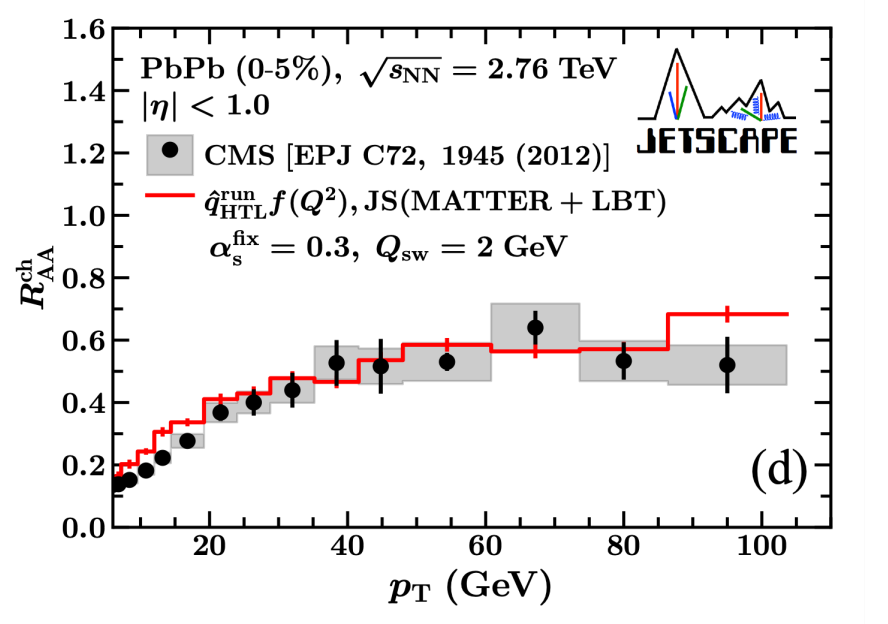
\includegraphics[width=\textwidth]{charged-hadron-RAA.png}};
    \end{tikzpicture}
  \end{columns}
\end{frame}
